% Integration snippets for director-helper-3; paths resolve from docs/analysis-note, including its blinded copies.
\begin{figure*}[tb]
\centering
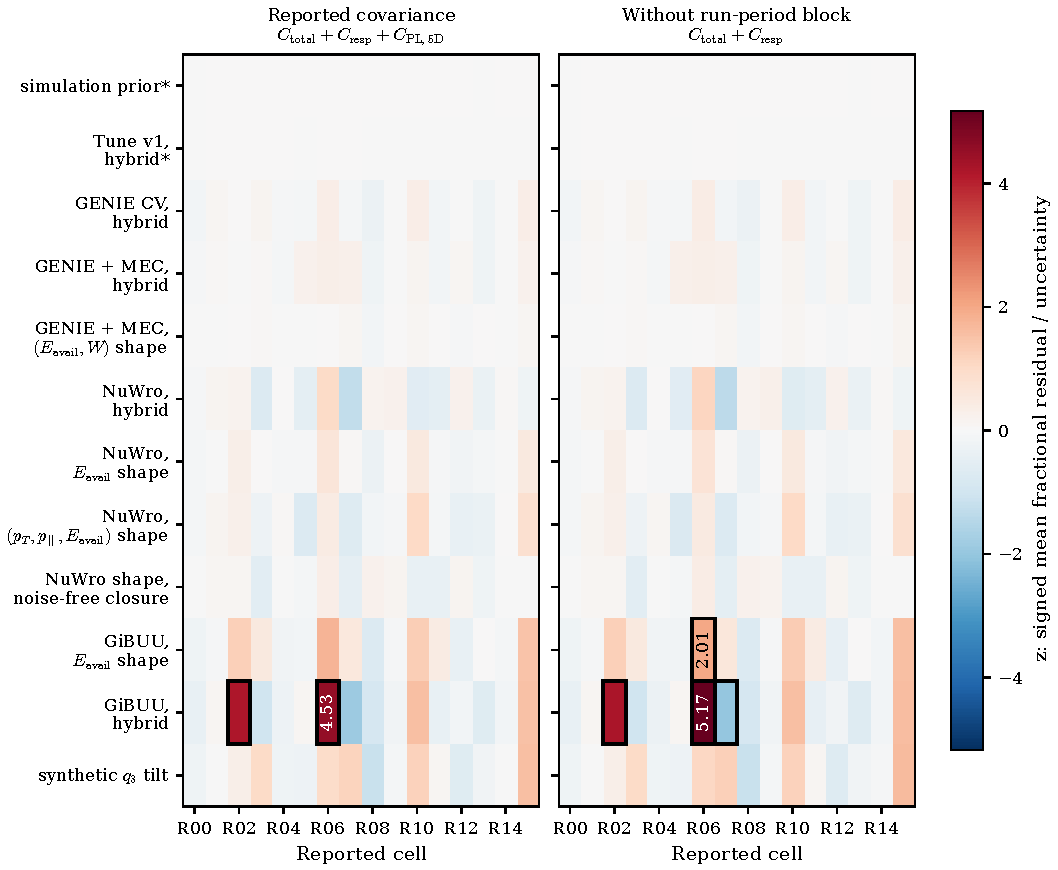
\includegraphics[width=\textwidth]{figures/methods_short/paper_bias_cells.pdf}
\caption{Fake-data bias of the reported five-observable estimator on the sixteen cells, at the twelve graded truths of table~\ref{tab:fd16}, in the same order. Color gives the signed residual $z$, the mean fractional residual, (unfolded $-$ true)/true, divided by its uncertainty $\sqrt{\mathrm{diag}(C+N)}$, where $N$ is the noise covariance of that mean. The noise-free closure uses its single residual and $N=0$. Left panel: the reported covariance, $C_{\mathrm{total}}+C_{\mathrm{resp}}+C_{\mathrm{PL,5D}}$. Right panel: the covariance without the run-period block. The table's $C_{\mathrm{total}}$-only reading is not shown. Each covariance omits the truth's own generator component as in the table. Numbers label the cell with largest $|z|$ in each outlined row, to two decimals as in the table. Black outlines show only the per-cell criterion, $|z|>\fvval{trig-z}$. A truth can also be flagged by its $\chi^2$ $p$ value (table~\ref{tab:fd16}), as the synthetic $q_3$ tilt is under the reported covariance. The bias is identical in both panels; only the covariance differs. An asterisk marks the simulation's own truth. These tests assess only bias.}
\label{fig:bias-cells}
\end{figure*}
% Proposed citation: section 5.3, immediately before Table 2, retaining the complete table.

\begin{figure*}[tb]
\centering
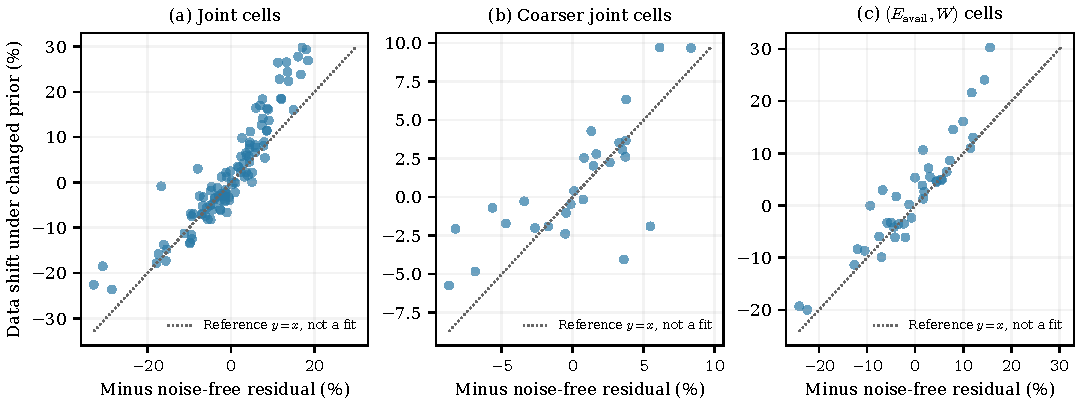
\includegraphics[width=\textwidth]{figures/methods_short/paper_prior_response.pdf}
% Sources: sec_5d.tex:204: "Strong correlation supplies no per-cell bound; shifts do not measure unknown real-data bias".
% Populations: app_statmethods_nd.tex:25, J/H2/EW = 109/27/39; verified by the pinned prior reduction.
\caption{Sensitivity to the prior of the reported five-observable estimator at five iterations. The vertical axis gives the fractional change of the data result, using the reported estimator with its background refinement, when the simulation prior is reweighted to the NuWro $(p_T,p_\parallel,E_{\mathrm{avail}})$ shape. The horizontal axis is minus the noise-free residual, (unfolded $-$ true)/true, at that changed truth: this comparator uses signal-only simulation, with no background refinement, whereas the data result uses the reported estimator's background refinement. Panels (a), (b) and (c) use the joint (J, 109), coarser joint (H2, 27) and $(E_{\mathrm{avail}},W)$ (EW, 39) cells defined in the companion note (\nsec{sec:gbdt-model-dependence}; \napp{sec:gbdt-diagnostic-definitions}); no panel is the sixteen-cell result. Points are cells, not independent repeated experiments. The dotted line is $y=x$, for reference, with no fit. The shifts measure sensitivity to the prior, not a measured bias of the data result. The correlation supplies no per-cell bias bound (\nsec{sec:gbdt-model-dependence}).}
\label{fig:prior-response}
\end{figure*}
% Proposed citation: section 7, after the sentence saying these shifts measure sensitivity to the prior.


% Source: a3-rounding-shifts-20261109/README.md CITABLE FOR and cluster CSV/JSON,
% merged at 13d714bf; s5e_analyze_candidate.py:147-154; amendment 3 A3 criteria.
% Proposed citation: section 6.1, after the sentence giving median 0.8 and maximum 2.6.
% director-helper-3 chooses the float placement for the paper and blinded copy.
\begin{figure}
\centering
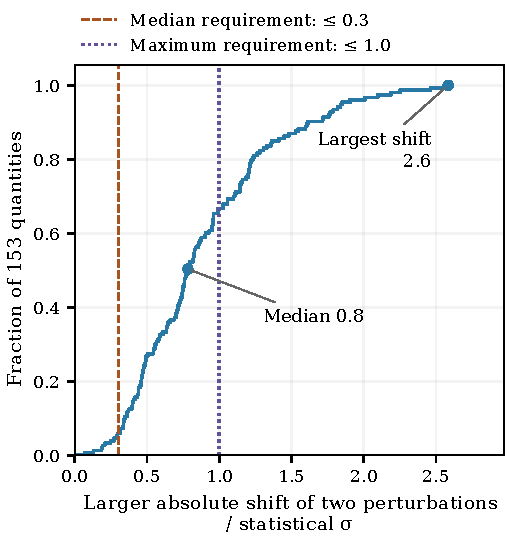
\includegraphics[width=\linewidth]{figures/methods_short/paper_rounding_shifts.pdf}
\caption{Numerical instability of the reported five-observable estimator. The cumulative distribution shows, for each of the 153 quantities, the larger absolute shift under two rounding-level perturbations of the data, divided by its data-bootstrap statistical standard deviation. The quantities are the 109 joint-cell integrals, 42 $(E_{\mathrm{avail}},W)$ quantities and two totals. Perturbations move inputs within half a float32 unit in the last place while preserving their grid membership; the reference is the same input values represented in float64. The statistical standard deviation is estimated from 100 refitted data-bootstrap replicas. Vertical lines mark the requirements fixed before the test: at most 0.3 statistical standard deviations for the median and 1.0 for the maximum. The observed median and the largest shift, in J145, are marked. Points in this distribution are different quantities, not repeated experiments.}
\label{fig:rounding-shifts}
\end{figure}
